\section{Driving the atom with a laser}
Se consider how a laser drives a two-level atom. Note that for simplicity we will ignore the interaction 
of the atom with the quantized EM field modes- this is for us to be able to focus on the atom-laser 
interaction (even though the quantized field and its effects are always present).
\begin{figure}[htbp]
    \centering
    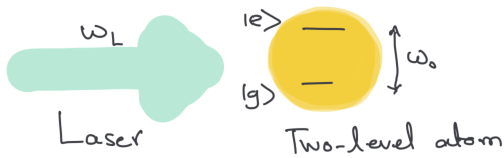
\includegraphics[width=.4\columnwidth]{PartOne/ChapterFour/figures/drivingtheatom.png}
    \caption{Driving the atom (two-level) with a laser.}
\end{figure}

The Hamiltonian for the total system is:
\begin{align}
    H=H_A+H_{AL},\quad \begin{array}{l}
        H_A=\hbar\omega_0\hsigma_+\hsigma_-\\
        H_{AL}=-\hbd\cdot\bE_L(\br_A,t)
    \end{array}
\end{align}
The E-field is:
\begin{align*}  
    \hE_L(\br_A,t)=\E_Le^{-i(\omega_Lt-\bk_L\cdot\br_A)}+\E_L^*e^{i(\omega_Lt-\bk_L\cdot\br_A)}
\end{align*}
\begin{align*}
    H_{AL}=-\left[\bd\hsigma_++\bd^*\hsigma_-\right]\cdot\left[\E_Le^{-i(\omega_Lt-\bk_L\cdot\br_A)}+\E_L^*e^{i(\omega_Lt-\bk_L\cdot\br_A)}\right].
\end{align*}
Moving to the interaction picture with respect to $H_A$, assuming $\br_A=0$ 
\begin{align}
    \tilde{\sigma}_\pm=e^{iH_At/\hbar}\hsigma_\pm e^{-iH_At/\hbar}=\hsigma_\pm e^{\pm i\omega_0t}.
\end{align}
The Hamiltonian in the interaction picture is:
\begin{align*}
    \tilde{H}_{AL}&=e^{iH_At/\hbar}H_{AL}e^{-iH_At/\hbar}=-\left[\bd\hsigma_+e^{i\omega_0t}+\bd^*\hsigma_-e^{-i\omega_0t}\right]\cdot\left[\E_Le^{-i\omega_Lt}+\E_L^*e^{i\omega_Lt}\right].
\end{align*}
Making the RWA:
\begin{align*}
    \tilde{H}_{AL}=-\left[\bd\cdot\E_L\hsigma_+e^{i(\omega_0-\omega_L)t}+\bd^*\cdot\E_l^*\hsigma_-e^{-i(\omega_0-\omega_L)t}\right]\approx\frac{\hbar}{2}
    (\Omega\hsigma_+e^{-i\Delta_Lt}+\Omega^*\hsigma_-e^{i\Delta_Lt}).
\end{align*}
We identify two things:
\begin{align}
    \text{Raby frequency}:\qquad \frac{1}{2}\hbar\Omega=-\bd\cdot\E_l,\quad\text{and}\quad\text{Detuning}:\qquad\Delta_L=\omega_L-\omega_0.
\end{align}
Let us consider the evolution of the atomic state via the Schrodinger equation:
\begin{align*}
    i\hbar\partial_t\ket{\Psi(t)}_I&=\tilde{H}_{AL}\ket{\Psi(t)}_I\\
    i\hbar\frac{d}{dt}\left[c_g(t)\ket{g}+c_e(t)\ket{e}\right]&=\frac{\hbar}{2}\left[\Omega\hsigma_+e^{-i\Delta_Lt}+\Omega^*\hsigma_-e^{i\Delta_Lt}\right]
    \cdot\left[c_g(t)\ket{g}+c_e(t)\ket{e}\right]\\
    i\left[\frac{dc_g}{dt}\ket{g}+\frac{dc_e}{dt}\ket{e}\right]&=\frac{\Omega}{2}c_ge^{-i\Delta_Lt}\ket{e}+\frac{\Omega^*}{2}c_ee^{i\Delta_Lt}\ket{g},\quad(\hsigma_+\ket{g}=\ket{e},\hsigma_-\ket{e}=\ket{g}).
\end{align*}
Equating coefficients of $\ket{g}$ and $\ket{e}$ yields:
\begin{align}
    \text{Equation of motions}\qquad\highlight{
    \begin{array}{l}
        \displaystyle\frac{dc_g}{dt}=-i\frac{\Omega^*}{2}c_ee^{i\Delta_Lt}\\
        \displaystyle\frac{dc_e}{dt}=-i\frac{\Omega}{2}c_ge^{-i\Delta_Lt}
    \end{array}}
\end{align}

Let us first consider the case when the laser is at resonance with the atomic transition frequency, that is, $\Delta_L=0$.
\begin{align*}
    \frac{dc_g}{dt}=-i\frac{\Omega^*}{2}c_e,\;\frac{dc_e}{dt}=-i\frac{\Omega}{2}c_g\Longrightarrow\frac{d^2c_e}{dt^2}=-\frac{|\Omega|^2}{4}c_e.
\end{align*}
The solution of this expression is:
\begin{align}
    c_e(t)=A\cos\left(\frac{|\Omega|t}{2}\right)+B\sin\left(\frac{|\Omega|t}{2}\right).
\end{align}
The coefficients are found as:
\begin{align*}
    t=0:&\quad c_e(0)=A\\
    t=0':&\quad \frac{dc_e}{dt}(0)=-i\frac{\Omega}{2}c_g(0)=\frac{B|\Omega|}{2}\longrightarrow B=-i\frac{\Omega}{|\Omega|}c_g(0).
\end{align*}
The probability amplitude for being in the excited and ground states are:
\begin{align}
    c_e(t)&=c_e(0)\cos\left(\frac{|\Omega|t}{2}\right)-\frac{i\Omega}{|\Omega|}c_g(0)\sin\left(\frac{|\Omega|t}{2}\right),\\
    c_g(t)&=c_g(0)\cos\left(\frac{|\Omega|t}{2}\right)-\frac{i\Omega^*}{|\Omega|}c_e(0)\sin\left(\frac{|\Omega|t}{2}\right)
\end{align}
This is the general dynamics of a laser-driven two-level atom. 

Let us now considee that the atom is initially in the ground state and $\Omega=\Omega^*=|\Omega|$:
\begin{align*}
    c_g(t)=\cos\left(\frac{\Omega t}{2}\right),\quad c_e(t)=-i\sin\left(\frac{\Omega t}{2}\right).
\end{align*}
Probability of finding the atom in the ground or excited states are:
\begin{align*}
    P_g=|c_g(t)|^2=\cos^2\left(\frac{|\Omega|t}{2}\right),\quad P_e=|c_e(t)|^2=\sin^2\left(\frac{|\Omega|t}{2}\right).
\end{align*}
The following figure illustrates the evolution of ground and excited states. We see that population of the atom oscilatess between those levels at a 
frequency $\Omega$, called \bfemph{Rabi frequency}. This phenomenon is called \bfemph{Rabi flopping}.
\begin{figure}[htbp]
    \centering
    \begin{subfigure}{.45\columnwidth}
        \centering
        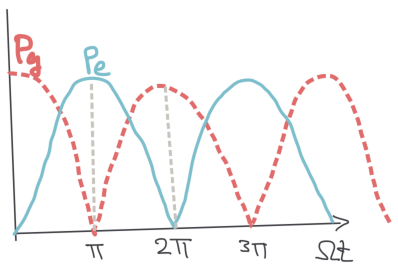
\includegraphics[width=.8\columnwidth]{PartOne/ChapterFour/figures/rabiflopping.png}
        \caption{Time evolution of states}
    \end{subfigure}
    \hfill
    \begin{subfigure}{.45\columnwidth}
        \centering
        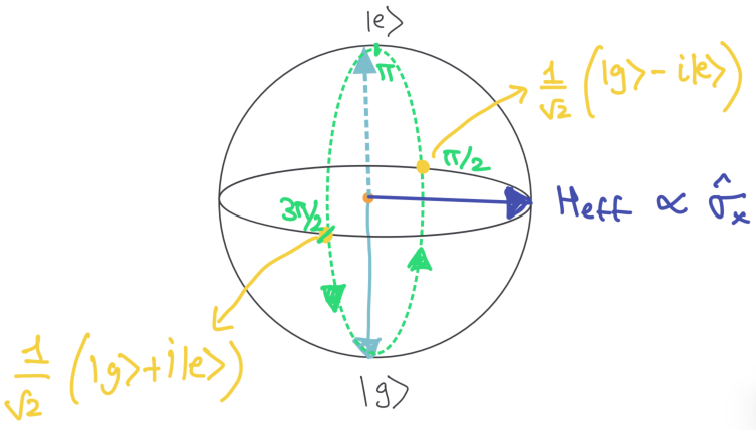
\includegraphics[width=.9\columnwidth]{PartOne/ChapterFour/figures/rabiflopping_bloch.png}
        \caption{Bloch sphere}
    \end{subfigure}
    \caption{Rabi flopping from initial ground state.}
\end{figure}

Inceease in excited state population corresponds to laser absorption and decrease in excited state implies stimulatred emission. In particular,
\begin{itemize}[itemsep=0pt,topsep=0pt,parsep=0pt]
    \item $\Omega t=\pi$ The atom in the ground state ends up in the excited state: $\pi$-pulse.
    \item $\Omega t=\pi/2$ The atom ends up in a superposition of $(1/\sqrt{2})(\ket{g}-i\ket{e})$: $\pi/2$-pulse. 
\end{itemize}
We can depict this evolution of the atomic state in the BLoch sphere. The state preceses around the Hamiltonian vector $H_{eff}$ with a frequency 
$|\Omega|/2$.


%%
\subsection{Dressed states}
Let us look at the equations of motion:
\begin{align*}
    \begin{array}{l}
        \displaystyle\frac{dc_g}{dt}=-i\frac{\Omega^*}{2}c_ee^{i\Delta_Lt}\\
        \displaystyle\frac{dc_e}{dt}=-i\frac{\Omega}{2}c_ge^{-i\Delta_Lt}
    \end{array}\longrightarrow
    \begin{array}{l}
        \displaystyle\frac{dc_g}{dt}e^{-i\Delta_Lt/2}=-i\frac{\Omega^*}{2}c_ee^{i\Delta_Lt/2}\\
        \displaystyle\frac{dc_e}{dt}e^{i\Delta_Lt/2}=-i\frac{\Omega}{2}c_ge^{-i\Delta_Lt/2}
    \end{array}.   
\end{align*}
For a finite detuning $\Delta_L$, let us define 
\begin{align}
    \tilde{c}_e=c_ee^{i\Delta_Lt/2},\quad\tilde{c}_g=c_ge^{-i\Delta_Lt/2}.
\end{align}
This allows us to rewrite the coupled differential equations without any explicit time dependence:
\begin{align*}
    \frac{d\tilde{c}_e}{dt}&=\frac{dc_e}{dt}e^{i\Delta_Lt/2}+\frac{i\Delta_L}{2}c_ee^{i\Delta_Lt/2}=-\frac{i\Omega}{2}c_ge^{i\Delta_Lt/2}+\frac{i\Delta_L}{2}\tilde{c}_e=
    -\frac{i\Omega}{2}\tilde{c}_g+\frac{i\Delta_L}{2}\tilde{c}_e\\
    \frac{d\tilde{c}_g}{dt}&=\frac{dc_g}{dt}e^{-i\Delta_Lt/2}-\frac{i\Delta_L}{2}c_ge^{-i\Delta_Lt/2}=-\frac{i\Omega}{2}\tilde{c}_e-\frac{i\Delta_L}{2}\tilde{c}_g.
\end{align*}
Then,
\begin{align}
    \frac{d}{dt}\begin{bmatrix}
        \tilde{c}_e\\\tilde{c}_g
    \end{bmatrix}=-\frac{i}{\hbar}\begin{bmatrix}
        -\hbar\Delta_L/2&\hbar\Omega/2\\\hbar\Omega/2&\hbar\Delta_L/2
    \end{bmatrix}\begin{bmatrix}
        \tilde{c}_e\\\tilde{c}_g
    \end{bmatrix}\Longrightarrow \frac{d}{dt}\bm{c}=-\frac{i}{\hbar}H_{\mathrm{eff}}\bm{c}.
\end{align}
One can diagonalize the above Hamiltonian such that 
\begin{align*}
    V\frac{d\bm{C}}{dt}&=-\frac{i}{\hbar}\underbrace{VH_{eff}V^{-1}}_{H_{eff,D}}\underbrace{V\bm{C}}_{\text{New eigenstates}}\\
    \frac{d}{dt}\underbrace{\begin{bmatrix}
        C_+\\C_-
    \end{bmatrix}}_{V\bm{C}}&=-\frac{i}{\hbar}\begin{bmatrix}
        E_+&0\\0&E_-
    \end{bmatrix}\underbrace{\begin{bmatrix}
        C_+\\C_-
    \end{bmatrix}}_{V\bm{C}}.
\end{align*}
Then, the dressed eigenstates are:
\begin{align}
    \text{Dessed eigenstates}\qquad\begin{array}{l}
        \ket{+}=\cos\theta\ket{e}+\sin\theta\ket{g}\\
        \ket{-}=-\sin\theta\ket{e}+\cos\theta\ket{g}
    \end{array},\quad\tan2\theta=-\frac{\Omega}{\Delta_L}.
\end{align}
The atomic state expressed in dresses basis:
\begin{align*}
    \ket{\Psi(t)}=c_+\ket{+}+c_-\ket{-},\quad\begin{array}{l}
        c_+(t)=c_+(0)e^{-iE_+t/\hbar}\\
        c_-(t)=c_-(0)e^{-iE_-t/\hbar}
    \end{array},\quad E_\pm=\pm\frac{\hbar}{2}\sqrt{\Delta_L^2+\Omega^2}.
\end{align*}
A qualitative evolution is given in the following figure.
\begin{figure}[H]
    \centering
    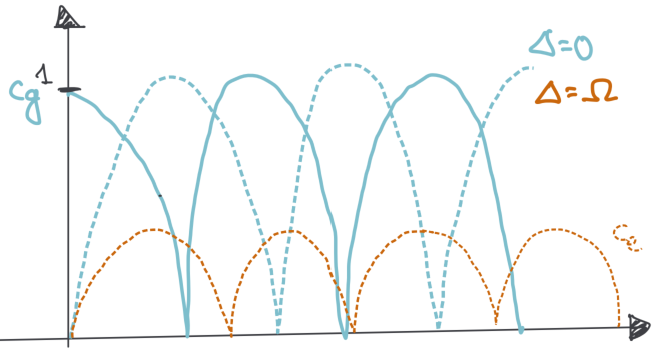
\includegraphics[width=.4\columnwidth]{PartOne/ChapterFour/figures/evolution_dressedstates.png}
    \caption{Evolution of $c_g$ and $c_e$ for different detuning values $\Delta_L$.}
\end{figure}
%%
\subsection{Dressed states and energies variation with $\Delta_L$}
The angle $\theta$ is:
\begin{align*}
    \tan2\theta=-\frac{\Omega}{\Delta_L}\longrightarrow2\theta=-\underbrace{\tan^{-1}\left(\frac{\Omega}{\Delta_L}\right)}_{[0,\pi]}
\end{align*}
Then, for different ragions of the detuning we have:
\begin{figure}[H]
    \centering
    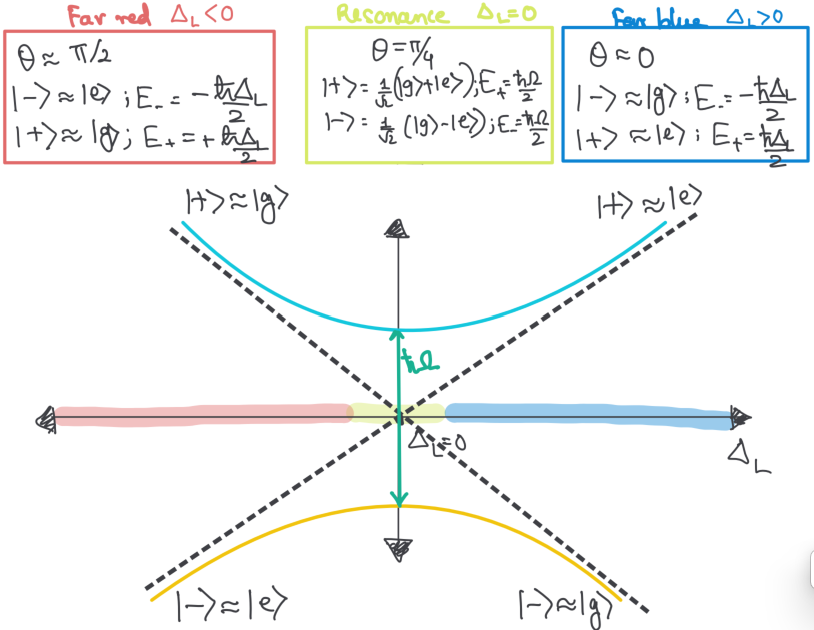
\includegraphics[width=.6\columnwidth]{PartOne/ChapterFour/figures/dressedstates_variation.png}
    \caption{Chirping the external field slowly enough such that the atomic state remains in an eigenstate of the Hamiltonian.}
\end{figure}

It can be shown that the probability of graing from the ground to excited state is:
\begin{align}
    P_e(t\to\infty)=1-\exp\left(-\frac{\pi\Omega^2}{2|\partial_t\Delta_L|}\right).
\end{align}
This effect is referred to as \bfemph{adiabatic passage}.


